\begin{frame}{Contents}
\tableofcontents
\end{frame}

\section{Basics}

\begin{frame}[t,fragile]{What is a Digital Image?}
    \begin{columns}[t]
        \column{0.6\textwidth}
        \begin{itemize}
            \item A grayscale digital image is a rectangular array of numbers which represent pixels.
            \item Each pixel can take an integer  value in the range \fillblank{ $[0, 255]$ }, for an 8-bit image.
            \item If the image is a color image, then there would be three such arrays.
            \item The size of this array is actually the resolution of the image, e.g., example, $3048\times2248$.
            \item We take the top-left pixel as the $(0,0)$ pixel and vertical axis as the \fillblank{$i$} axis.
        \end{itemize}
        \column{0.4\textwidth}
            \begin{figure}
              \centering
                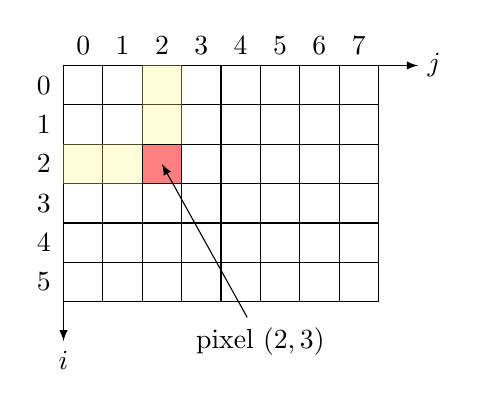
\begin{tikzpicture}[scale=0.5]
	\foreach \i in {0,1,...,6}
	{
		\draw (0,\i) -- ++(8,0);
	}
	\foreach \i in {0,1,...,5}
	{
		\node at (-0.5, 5.5 - \i) {$\i$};
	}	
	\foreach \j in {0,1,...,8}
	{
		\draw (\j,0) -- ++(0,6);
	}
	\foreach \j in {0,1,...,7}
	{
		\node at (\j + 0.5, 6.5) {$\j$};
	}		
	\draw[-latex] (0,6) -- ++(0,-7) node[anchor=north] {$i$};		
	\draw[-latex] (0,6) -- ++(9,0) node[anchor=west] {$j$};

    \pause
    \draw [draw=none, fill=yellow!50, opacity=0.3] (0,3) rectangle (3,4);
    \draw [draw=none, fill=yellow!50, opacity=0.3] (2,3) rectangle (3,6);
    \draw[fill=red!50] (2,3) rectangle ++(1,1);
    \node (a) at  (5,-1) {pixel $(2,3)$};
    \draw[-latex] (a) -- (2.5,3.5);
	
\end{tikzpicture} 
              \caption{A $6\times 8$ image}
            \end{figure}
    \end{columns}

\end{frame}


\begin{frame}[t,fragile]{What is a Color Digital Image?}
    \begin{columns}[t]
        \column{0.6\textwidth}
        \begin{itemize}
            \item The grayscale image that we considered s a two-dimensional array, or a single plane.
            \item A color image has three such planes, one for blue, one for green and one for red. We call such an image an BGR image.
            \item If we access a pixel location such as $(2,3)$, we will get three values, B, G, and R.
            \item Each value is in $[0,255]$. In this context, \fillblank{$2^8 \times 2^8 \times 2^8$} different colors are possible.
        \end{itemize}
        \column{0.4\textwidth}
            \begin{figure}
              \centering
                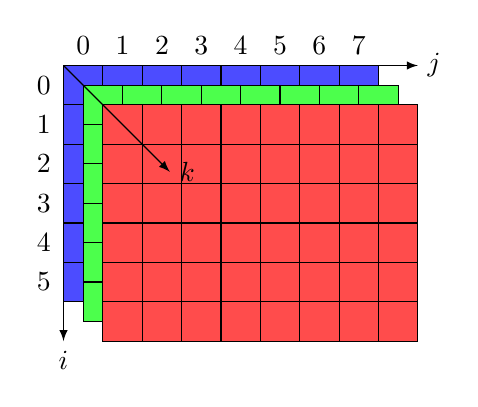
\begin{tikzpicture}[scale=0.5]
	\draw[fill=blue!70] (0,0) rectangle (8,6);
	\foreach \i in {0,1,...,6}
	{
		\draw (0,\i) -- ++(8,0);
	}
	\foreach \i in {0,1,...,5}
	{
		\node at (-0.5, 5.5 - \i) {$\i$};
	}	
	\foreach \j in {0,1,...,8}
	{
		\draw (\j,0) -- ++(0,6);
	}
	\foreach \j in {0,1,...,7}
	{
		\node at (\j + 0.5, 6.5) {$\j$};
	}		
	\draw[-latex] (0,6) -- ++(0,-7) node[anchor=north] {$i$};		
	\draw[-latex] (0,6) -- ++(9,0) node[anchor=west] {$j$};

\begin{scope}[xshift=0.5cm, yshift=-0.5cm]
	\draw[fill=green!70] (0,0) rectangle (8,6);
	\foreach \i in {0,1,...,6}
	{
		\draw (0,\i) -- ++(8,0);
	}

	\foreach \j in {0,1,...,8}
	{
		\draw (\j,0) -- ++(0,6);
	}

\end{scope}


\begin{scope}[xshift=1cm, yshift=-1cm]
	\draw[fill=red!70] (0,0) rectangle (8,6);
	\foreach \i in {0,1,...,6}
	{
		\draw (0,\i) -- ++(8,0);
	}

	\foreach \j in {0,1,...,8}
	{
		\draw (\j,0) -- ++(0,6);
	}

\end{scope}

\draw[-latex] (0,6) -- ++(2.7,-2.7) node[anchor=west] {$k$};
	
\end{tikzpicture} 
              \caption{A $6\times 8$ BGR image}
            \end{figure}
    \end{columns}

\end{frame}


\begin{frame}[fragile]{Code for Generating a $6\times 8$ Images}
\begin{columns}[t]
\column[t]{0.5\textwidth}
       \begin{lstlisting}[caption=A Grayscale Image, language=Python, escapechar=\@]
%matplotlib inline
import cv2 as cv
import numpy as np
import matplotlib.pyplot as plt
@\fillblank{im = np.zeros((6,8),dtype=np.uint8)}@
@\fillblank{im[2,3] = 255}@
fig, ax = plt.subplots()
ax.imshow(im, cmap = 'gray')
ax.xaxis.tick_top()
plt.show()
        \end{lstlisting}
\column[t]{0.5\textwidth}
       \begin{lstlisting}[caption=A Color Image,language=Python, escapechar=\@]
%matplotlib inline
import cv2 as cv
import numpy as np
import matplotlib.pyplot as plt
@\fillblank{im = np.zeros((6,8, 3),dtype=np.uint8)}@
@\fillblank{im[2,3] = [255, 255, 100]}@
print(im[2,3])
fig, ax = plt.subplots()
ax.imshow(im, cmap = 'gray')
ax.xaxis.tick_top()
plt.show()
         \end{lstlisting}
\end{columns}
\end{frame}




\begin{frame}[t, fragile]{Opening and Displaying  Images}
    \begin{enumerate}
      \item We can use OpenCV to open and display images. We can examine the size (resolution) of the image as well.
    \end{enumerate}
\begin{columns}[t]
\column[t]{0.5\textwidth}
       \begin{lstlisting}[caption=Displaying Using Matplotlib, language=Python, escapechar=\@]
%matplotlib inline
import cv2 as cv
import matplotlib.pyplot as plt
img = cv.imread('../images/gal.jpg', cv.IMREAD_COLOR)
@\fillblank{img = cv.cvtColor(img, cv.COLOR\_BGR2RGB)}@
@\fillblank{fig, ax = plt.subplots()}@
@\fillblank{ax.imshow(img)}@
@\fillblank{ax.set\_title('Image')}@
@\fillblank{plt.show()}@
        \end{lstlisting}
\column[t]{0.5\textwidth}
       \begin{lstlisting}[caption=Displaying Using OpenCV,language=Python, escapechar=\@]
import cv2 as cv
import matplotlib.pyplot as plt
img = cv.imread('../images/katniss.jpg', cv.IMREAD_COLOR)
@\fillblank{cv.namedWindow('Image', cv.WINDOW\_NORMAL)}@
@\fillblank{cv.imshow('Image', img)}@
@\fillblank{cv.waitKey(0)}@
@\fillblank{cv.destroyAllWindows()}@
         \end{lstlisting}
\end{columns}
Q:Why do we need to \lstinline!cv.cvtColor! only when displaying using Matplotlib?
\end{frame}



\begin{frame}[t, fragile]{Displaying  Image Properties}
    \begin{lstlisting}[caption=Displaying  Image Properties, language=Python, escapechar=\@]
%matplotlib inline
import cv2 as cv
import matplotlib.pyplot as plt
img = cv.imread('../images/hugh.jpg', cv.IMREAD_COLOR)
img = cv.cvtColor(img, cv.COLOR_BGR2RGB)
fig, ax = plt.subplots()
ax.imshow(img)
ax.set_title('Image')
plt.show()
@\fillblank{print(img.shape)}@
@\fillblank{print(img.size)}@
@\fillblank{print(img.dtype)}@
    \end{lstlisting}
\end{frame}



\begin{frame}[t, fragile]{Increasing the Brightness Using OpenCV}
    \begin{lstlisting}[caption=Increasing the Brightness Using OpenCV, language=Python, escapechar=\@]
import cv2 as cv
import matplotlib.pyplot as plt
img = cv.imread('../images/keira.jpg', cv.IMREAD_GRAYSCALE)
@\fillblank{imgb = img + 100}@
@\fillblank{imgc = cv.add(img, 100)}@
f, ax = plt.subplots(1,3)
ax[0].imshow(img, cmap="gray")
ax[0].set_title('Original')
ax[1].imshow(imgb, cmap="gray")
ax[1].set_title('img + 100')
ax[2].imshow(imgc, cmap="gray")
ax[2].set_title('cv.add')
    \end{lstlisting}
\begin{itemize}
    \item What is the reason for the \lstinline!img + 100! operation to be incorrect?
\end{itemize}
\end{frame}

\begin{frame}[t, fragile, allowframebreaks]{Increasing the Brightness Using Loops}
    \begin{lstlisting}[caption=Increasing the Brightness Using Loops, language=Python, escapechar=\@]
import cv2 as cv
import matplotlib.pyplot as plt
import numpy as np
@\fillblank{def image\_brighten(image, shift):}@
    @\fillblank{h = image.shape[0]}@
    @\fillblank{w = image.shape[1]}@
    @\fillblank{result = np.zeros(image.shape, image.dtype)}@
    @\fillblank{for i in range(0,h):}@
        @\fillblank{for j in range(0,w):}@
            @\fillblank{no\_overflow = True if image[i,j] + shift < 255 else False}@
            @\fillblank{result[i,j] = min(image[i,j] + shift, 255) if no\_overflow else 255}@
    return result

img = cv.imread('../images/keira.jpg', cv.IMREAD_GRAYSCALE)
%timeit imgb = image_brighten(img, 200)
f, ax = plt.subplots(1,2)
ax[0].imshow(img, cmap = 'gray')
ax[0].set_title('Original')
ax[1].imshow(imgb, cmap = 'gray')
ax[1].set_title('image_brighten')
    \end{lstlisting}
\begin{itemize}
    \item Do not use this, due to inefficiencies. Instead, use OpenCV filters or Cython (?).
    \item In the convolution operations---which we would cover later---to produce each output pixel, we need to multiply and add, say, a $3\times 3$ neighborhood of pixels. How many loops would this require? What is the computational complexity?
\end{itemize}
\end{frame}


\begin{frame}[t, fragile]{Zeroing Out Green and Blue Planes}
    \begin{lstlisting}[caption=Zeroing Out Green and Blue Planes, language=Python, escapechar=\@]
%matplotlib inline
import matplotlib.pyplot as plt
import cv2 as cv
img = cv.imread('images/tom.jpg', cv.IMREAD_ANYCOLOR)
if img is None:
    print('Image could not be read.')
    assert False
img = cv.cvtColor(img, cv.COLOR_BGR2RGB)
plt.imshow(img)
plt.title('Image')
plt.xticks([]), plt.yticks([])
plt.show()
@\fillblank{img[:,:,1:3] = 0}@
plt.imshow(img)
plt.title('After Zeroing Planes')
plt.xticks([]), plt.yticks([])
plt.show()
    \end{lstlisting}


\end{frame}


\begin{frame}{Summary}
    \begin{enumerate}
      \item A grayscale digital image is an array of 8-bit unsigned integers in $[0,255]$. We call each integer a pixel.
      \item Color images have three such arrays (planes), one for red, one for green, and one for blue.
      \item We can manipulate an image using OpenCV function or a pair of for-loops to access each pixel (slower).
    \end{enumerate}
\end{frame}







\section{Intensity Transformations}




\begin{frame}{Intensity Transformations (Point Operations): Introduction}
    \begin{columns}[t]
        \column{0.6\textwidth}
        \begin{itemize}
          \item In intensity transformations, the output value of the pixel depends only on the \fillblank{input values of that pixel}, not it neighbors.
          \item Input image: $f(\vec{x})$\par Output image: $g(\vec{x})$ \par Intensity transform $g(\vec{x}) = T(f(\vec{x}))$
          \item E.g., \fillblank{identity transform $T(.) = 1$}
        \end{itemize}
        \column{0.4\textwidth}
        \begin{figure}
          \centering
            \begin{tikzpicture}
	\begin{axis}
	[
		xmin = 0,
		xmax = 255,
		ymin = 0,
		ymax = 255,
		xtick = {0, 50, 100, 150, 200, 255},
		ytick = {0, 50, 100, 150, 200, 255},	
		xlabel = {$f(\vec{x})$},	
		ylabel = {$g(\vec{x})$},
		axis equal,
		width=\textwidth,
		height=\textwidth,		
	]
	\addplot [mark=none, thick, blue!80] coordinates {
		(0,0)
		(255,255)
	};		
	\end{axis}
\end{tikzpicture} 
          \caption{Identity transform}
        \end{figure}
    \end{columns}

\end{frame}


\begin{frame}[t, fragile, allowframebreaks]{Intensity Transforms: Identity Transformation Code}
    \begin{lstlisting}[caption=Identity Transformation, language=Python, escapechar=\@]
%matplotlib inline
import cv2 as cv
import numpy as np
import matplotlib.pyplot as plt
@\fillblank{transform = np.arange(0, 256).astype('uint8')}@
fig, ax = plt.subplots()
ax.plot(transform)
ax.set_xlabel(r'Input, $f(\mathbf{x})$')
ax.set_ylabel('Output, $\mathrm{T}[f(\mathbf{x})]$')
ax.set_xlim(0,255)
ax.set_ylim(0,255)
ax.set_aspect('equal')
plt.savefig('transform.png')
plt.show()
img_orig = cv.imread('../images/katrina.jpg', cv.IMREAD_GRAYSCALE)
print(img_orig.shape)
cv.namedWindow('Image', cv.WINDOW_AUTOSIZE)
cv.imshow('Image', img_orig)
cv.waitKey(0)
@\fillblank{image\_transformed = cv.LUT(img\_orig, transform)}@
cv.imshow('Image', image_transformed)
cv.waitKey(0)
cv.destroyAllWindows()
    \end{lstlisting}

\begin{itemize}
    \item Explain the line \lstinline!image_transformed = cv.LUT(img_orig, transform)!.
    \item This can be done using NumPy only as \lstinline!image_transformed = transform[img_orig]!. Explain this operation.
    \item What is $T()$ here?
\end{itemize}

\end{frame}


\begin{frame}{What Is This Transformation?}
    \begin{columns}[t]
        \column{0.6\textwidth}
        \begin{itemize}[<+->]
          \item $g(\vec{x}) = - f(\vec{x})$
          \item Implementation: \lstinline!transform = np.arange(255,-1, -1).astype('uint8')!.
        \end{itemize}
        \column{0.4\textwidth}
        \begin{figure}
          \centering
            \input{./figures/negative_transform}
          \caption{Negative transform}
        \end{figure}
    \end{columns}

\end{frame}




\begin{frame}[t, fragile, allowframebreaks]{Intensity Transforms: Intensity Windowing }
    \begin{lstlisting}[caption=Intensity Windowing, language=Python, escapechar=\@]
%matplotlib inline
import cv2 as cv
import numpy as np
import matplotlib.pyplot as plt
c = np.array([(100, 50), (150, 200)])
@\fillblank{t1 = np.linspace(0, c[0,1], c[0,0] + 1 - 0).astype('uint8')}@
print(len(t1))
@\fillblank{t2 = np.linspace(c[0,1] + 1, c[1,1], c[1,0] - c[0,0]).astype('uint8')}@
print(len(t2))
@\fillblank{t3 = np.linspace(c[1,1] + 1, 255, 255 - c[1,0]).astype('uint8')}@
print(len(t3))
@\fillblank{transform = np.concatenate((t1, t2), axis=0).astype('uint8')}@
@\fillblank{transform = np.concatenate((transform, t3), axis=0).astype('uint8')}@
print(len(transform))
fig, ax = plt.subplots()
ax.plot(transform)
ax.set_xlabel(r'Input, $f(\mathbf{x})$')
ax.set_ylabel('Output, $\mathrm{T}[f(\mathbf{x})]$')
ax.set_xlim(0,255)
ax.set_ylim(0,255)
ax.set_aspect('equal')
plt.savefig('transform.png')
plt.show()
img_orig = cv.imread('../images/katrina.jpg', cv.IMREAD_GRAYSCALE)
cv.namedWindow("Image", cv.WINDOW_AUTOSIZE)
cv.imshow("Image", img_orig)
cv.waitKey(0)
image_transformed = cv.LUT(img_orig, transform)
cv.imshow("Image", image_transformed)
cv.waitKey(0)
cv.destroyAllWindows()
    \end{lstlisting}

\begin{itemize}
    \item What is $T()$ here?
\end{itemize}
        \begin{figure}
          \centering
            \input{./figures/intensity_windowing}
          \caption{Intensity windowing.}
        \end{figure}
\end{frame}




\begin{frame}{Histograms}
    \begin{enumerate}
      \item We can represent the intensity distribution over the range of intensities $[0,255]$, using a histogram.

    \item \fillblank{If $h$ is the histogram of a particular image, $h(r_k)$ gives us how many pixels have the intensity $r_k$. The histogram of a digital image with gray values in the range $[0, L-1]$ is a discrete function $h(r_k) = n_k$ where $r_k$ is the $k$th gray level and $n_k$ is the number of pixels having gray level $r_k$.}

    \item We can normalize the histogram by dividing by the total number of pixels $n$. Then we have an estimate of the probability of occurrence of level $r_k$, i.e., $p(r_k) = n_k/n$.

    \item The histogram that we described above has $L$ bins. We can construct a coarser histogram by selecting a smaller number of bins than $L$. Then several adjacent values of $k$ will be counted for a bin.

    \end{enumerate}
\end{frame}

\begin{frame}{Activity}
    \begin{enumerate}
      \item The figure shows a $3\times 4$ image. The range of intensities that this image has is $[0,7]$. Compute its histogram.
    \end{enumerate}
        \begin{figure}
          \centering
            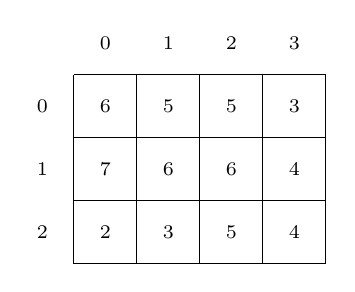
\begin{tikzpicture}[x=0.8cm, y=0.8cm]
%Ranga Rodrigo
%December 1, 2017
\def\rows{3}
\def\cols{4}
\def\printindices{false}
\def\printimagevalues{true}

\begin{filecontents*}{interpimage.dat}
2
3
5
4
7
6
6
4
6
5
5
3
\end{filecontents*}



\foreach \i in {0,1, ..., \rows}
{
	\draw[black] (0, \i)  -- ++(\cols, 0);
}
\foreach \j in {0,1, ..., \cols}
{
	\draw[black] (\j, 0)  -- ++(0, \rows);
}


\pgfmathsetmacro{\rowsminusone}{\rows -1 }%
\pgfmathsetmacro{\colsminusone}{\cols -1 }%


\ifthenelse{\equal{\printindices}{true}}
{
	\foreach \i in {0,1, ..., \rowsminusone}
	{
			\node at (-0.5, \rowsminusone - \i + 0.5) {\scriptsize{\i}};
	}
	
	\foreach \j in {0,1, ..., \colsminusone}
	{
			\node at (\j + 0.5, \rows + 0.5) {\scriptsize{\j}};
	}
}
{}

\ifthenelse{\equal{\printimagevalues}{true}}
{
	\pgfplotstableread{interpimage.dat}{\imagevalues}
	
	\foreach \i in {0,1, ..., \rowsminusone}
	{
		\foreach \j in {0,1, ..., \colsminusone}
		{	
			\pgfmathsetmacro{\index}{\i*\cols+\j}%
			\pgfplotstablegetelem{\index}{[index] 0}\of{\imagevalues}%
			\let\imagevalue\pgfplotsretval%
			 \node at (\j + 0.5,  \i + 0.5) {\scriptsize {$\imagevalue$}};
		}
	}
}
{}
\end{tikzpicture}

          \caption{Image for histogram computation.}
        \end{figure}

\end{frame}


\begin{frame}[t, fragile]{Histograms Using OpenCV}
\begin{columns}[t]
\column[t]{0.5\textwidth}
       \begin{lstlisting}[caption=Histogram of a Grayscale Image, language=Python, escapechar=\@]
import cv2 as cv
import numpy as np
import matplotlib.pyplot as plt
img = cv.imread('../images/gal.jpg', cv.IMREAD_GRAYSCALE)
@\fillblank{hist = cv.calcHist([img], [0], None, [256], [0,256])}@
plt.plot(hist)
plt.xlim([0,256])
plt.show()
        \end{lstlisting}
\column[t]{0.5\textwidth}
       \begin{lstlisting}[caption=Histogram of a Color Image,language=Python, escapechar=\@]
import cv2 as cv
import numpy as np
import matplotlib.pyplot as plt
img = cv.imread('../images/gal.jpg', cv.IMREAD_COLOR)
color = ('b', 'g', 'r')
@\fillblank{for i, c in enumerate(color):}@
@\fillblank{    hist = cv.calcHist([img], [i], None, [256], [0,256])}@
    plt.plot(hist, color = c)
    plt.xlim([0,256])
plt.show()
         \end{lstlisting}
\end{columns}
\end{frame}

\begin{frame}{Image Properties through Histograms}
    \begin{enumerate}
      \item If the image is dark histogram will have many values in the \fillblank{left} region, that correspond to  dark pixels.

      \item If the image is bright histogram will have many values in the \fillblank{right} region, that correspond to  bright pixels.

      \item If a significant number of pixels are dark and a significant number of pixels a bright, the histogram will have \fillblank{two} modes, one in the left region and the other in the right region.

      \item A \fillblank{flat} histogram signifies that the image has a uniform distribution of all intensities. Then, \fillblank{the contrast is high and image will look vibrant}.

    \end{enumerate}
\end{frame}


\begin{frame}{Histogram Equalization}
    \begin{enumerate}
      \item Photographers like to shoot pictures with a flat histogram, as such pictures are vibrant.

      \item Histogram equalization is \fillblank{a gray-level transformation that results in an image with a more or less flat histogram}.

      \item We can take and image and make its histogram flat by using the operation called histogram equalization.

    \end{enumerate}
\end{frame}

\begin{frame}[allowframebreaks]
	Consider, for now, that continuous intensity values of an image are to be processed. We assume that $r \in [0, L-1]$. Lets consider the intensity transformation
	\begin{equation}\label{eq:he01}
		s = T(r) \quad 0 \leq r \leq L -1
	\end{equation}
	that produces an output intensity level $s$ for every pixel in the input image having intensity $r$. We assume that	
\begin{itemize}
	\item $T(r)$ is \fillblank{monotonically increasing in the interval $0 \leq r \leq L -1$, and}
	\item \fillblank{$0 \leq T(r) \leq L -1$ for $0 \leq r \leq L -1$}.
\end{itemize}
The intensity levels in the image may be viewed as random variables in the interval $[0, L-1]$. Let $p_r(r)$ and $p_s(s)$ denote the probability density functions (PDFs) of $r$ and $s$. A fundamental result from basic probability theory is that if $p_r(r)$ and $T(r)$ are known, and $T(r)$ is continuous and differentiable over the range of values of interest, then the PDF of the transformed variable $s$ can be obtained using the simple formula
	\begin{equation}\label{eq:he02}
		\fillblank{p_s(s)  = p_r(r) \left|\frac{dr}{ds}\right|.}
	\end{equation}
	
Now let's consider the following transform function:
	\begin{equation}\label{eq:he03}
		\fillblank{s = T(r) =(L -1)\int_0^r p_r(w)dw,}
	\end{equation}
where $w$ is the dummy variable of integration. The right-hand side of this equation is the cumulative distribution function (CDF) of random variable $r$. This function satisfies the two conditions that we mentioned.
\begin{itemize}
	\item Because PDFs are always positive and the integral of a function is the area under the curve, Equation \ref{eq:he03} satisfies the first condition. This is because the area under the curve cannot decrease as $r$ increases.
	\item When the upper limit in this equation is $r= L-1$, the integral evaluates to 1, because the area under a PDF curve is always 1. So the maximum value of $s$ is $L-1$, and the second condition is also satisfied.
\end{itemize}
To find $p_s(s)$ corresponding to this transformation we use Equation \ref{eq:he01}.
	\begin{equation}\label{eq:he04}
		\begin{split}
		\frac{ds}{dr} &= \frac{dT(r)}{dr},\\
									&= \fillblank{(L-1) \frac{d}{dr}\left[\int_0^r p_r(w)dw\right]},\\
									&= \fillblank{(L-1) p_r(r)}.\\
		\end{split}
	\end{equation}
Substituting this result in Equation \ref{eq:he01}, and keeping in mind that all probability values are positive, yields
	\begin{equation}\label{eq:he04}
		\begin{split}
		p_s(s) &=  \fillblank{p_r(r) \left|\frac{dr}{ds}\right|},\\
									&= \fillblank{p_r(r) \left|\frac{1}{(L-1)p_r(r)}\right|},\\
									&= \fillblank{\frac{1}{L-1}\quad 0 \leq s \leq L -1}.\\
		\end{split}
	\end{equation}
	We recognize the form of $p_s(s)$ in the last line of this equation as a uniform probability density function.
	
	For discrete values, we deal with probabilities (histogram values) and the summation instead of probability density functions and integrals. The probability of occurrence of intensity level $r_k$ in a digital image is approximated by
	\begin{equation}\label{eq:he05}
		\fillblank{p_r(r_k) = \frac{n_k}{MN}\quad k = 0,1, \dots, L -1},
	\end{equation}
	where $MN$ is the total number of pixels in the image, $n_k$ is the number of pixels that have intensity $r_k$, and $L$ is the number of possible intensity levels in the image (e.g., 256). Recall that a plot of $p_r(r_k)$ versus $r_k$ is commonly referred to as a histogram.

The discrete form of the Equation \ref{eq:he02} is
	\begin{equation}\label{eq:he06}
		\begin{split}
		s_k &= \fillblank{T(r_k) = (L-1) \sum_{j=0}^{k}p_r(r_j)},\\
		  &= \fillblank{\frac{(L-1)}{MN} \sum_{j=0}^{k}n_j \quad k = 0,1, \dots, L -1}.\\
		 \end{split}
	\end{equation}
	Thus the output image is obtained by mapping each pixel in the input image with intensity $r_k$ into a corresponding pixel level $s_k$ in the output image using Equation \ref{eq:he06}.
\end{frame}


\begin{frame}
	\begin{example}\label{ex:hemanual}
		Suppose that a 3-bit image ($L=8$) of size $64\times 64$ pixels ($MN=4096$) has the intensity distribution shown in Table \ref{ta:hemanual}, where the intensity levels are in the range $[0,L-1] = [0,7]$.  carry out histogram equalization.
	\end{example}
\end{frame}


\begin{frame}	
\begin{table}
	\centering
		\begin{tabular}{|c|c|c|c|c|c|}
		\hline
		$r_k$ & $n_k$ & $p_r(r_k) = n_k/MN$ & $\sum_{j=0}^k n_j$ & $\frac{(L-1)}{MN}\sum_{j=0}^k n_j$ & Rounded\\
		\hline		
        $r_0 = 0$ & 790 & 0.19 & & & \\
		\hline	
        $r_1 = 1$ & 1023 & 0.25 & & & \\
		\hline	
        $r_2 = 2$ & 850 & 0.21 & & & \\
		\hline	
        $r_3 = 3$ & 656 & 0.16 & & & \\
		\hline	
        $r_4 = 4$ & 329 & 0.08 & & & \\
		\hline	
        $r_5 = 5$ & 245 & 0.06 & & & \\
		\hline	
        $r_6 = 6$ & 122 & 0.03 & & & \\
		\hline	
        $r_7 = 7$ & 81 & 0.02 & & & \\
		\hline										
		\end{tabular}
	\caption{Table for Example \ref{ex:hemanual}.}
	\label{ta:hemanual}
\end{table}
\end{frame}



\begin{frame}[t, fragile, allowframebreaks]{Histogram Equalization }
    \begin{lstlisting}[caption=Histogram Equalization, language=Python, escapechar=\@]
import cv2 as cv
import numpy as np
from matplotlib import pyplot as plt
img = cv.imread('../images/shells.tif',cv.IMREAD_GRAYSCALE)

hist,bins = np.histogram(img.ravel(),256,[0,256])
cdf = hist.cumsum()
cdf_normalized = cdf * hist.max()/ cdf.max()
plt.plot(cdf_normalized, color = 'b')
plt.hist(img.flatten(),256,[0,256], color = 'r')
plt.xlim([0,256])
plt.legend(('cdf','histogram'), loc = 'upper left')
plt.title('Histogram of the Original Image')
plt.show()
@{\fillblank{equ = cv.equalizeHist(img)}@
hist,bins = np.histogram(equ.ravel(),256,[0,256])
cdf = @{\fillblank{hist.cumsum()}@
cdf_normalized = @{\fillblank{cdf * hist.max()/ cdf.max()}@
plt.plot(cdf_normalized, color = 'b')
plt.hist(equ.flatten(),256,[0,256], color = 'r')
plt.xlim([0,256])
plt.legend(('cdf','histogram'), loc = 'upper left')
plt.title('Histogram of the Equalized Image')
plt.show()
res = np.hstack((img,equ))
plt.axis('off')
plt.imshow(res, cmap='gray')
    \end{lstlisting}

\end{frame}


\begin{frame}{Histogram Equalization}

    \begin{figure}[ht]
      \centering
      \begin{subfigure}[b]{0.5\linewidth}
        \centering\includegraphics[width=100pt]{shells.png}
        \caption{Original image}\label{sf:shells}
      \end{subfigure}%
      \pause
      \begin{subfigure}[b]{0.5\linewidth}
        \centering\includegraphics[width=100pt]{shells_equalized.png}
        \caption{Histogram-equalized image}\label{sf:shells_equalized}
      \end{subfigure}
      \caption{Histogram Equalization}
    \end{figure}
\end{frame}




\begin{frame}{Power-Law Transformation (Gamma Correction)}
    \begin{columns}[t]
        \column{0.55\textwidth}
        \begin{equation*}
            \fillblank{g = f^\gamma, \quad f \in [0,1]}.
        \end{equation*}
        Values of $\gamma$ such that $0 < \gamma < 1$ map a narrow range of dark pixels to a wider range of dark pixels.\par
        $\gamma > 0$ has the opposite effect.\par
        $\gamma = 1$ gives the identity transform.
        \column{0.4\textwidth}
        \mode<beamer>
        {
        \begin{figure}
            \centering
            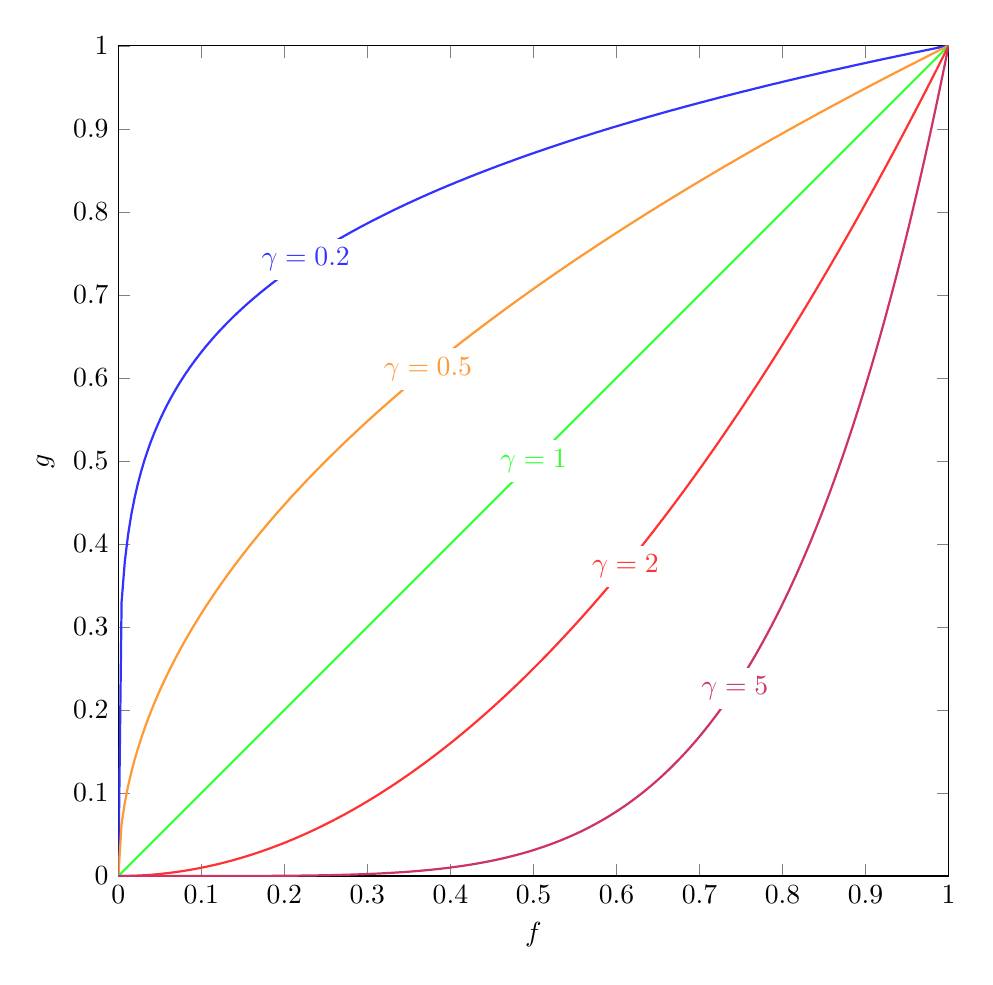
\begin{tikzpicture}
	\begin{axis}
	[
		xmin  = 0,
		xmax = 1,
		ymin = 0,
		ymax = 1,
		%enlarge limits=false,
		axis equal,
		xlabel = {$f$},
		ylabel = {$g$},		
    	legend style={at={(1.2,1)}, anchor=north,legend columns=1},	
		width=\textwidth,
		height=\textwidth    	
	]
	\addplot [domain = 0:1, samples=256, blue!80, thick]  {x^0.2} node[pos=0.5, fill=white] {$\gamma = 0.2$};
	\addplot [domain = 0:1, samples=256, orange!80, thick]  {x^0.5} node[pos=0.5, fill=white] {$\gamma = 0.5$};	
	\addplot [domain = 0:1, samples=256, green!80, thick]  {x^1} node[pos=0.5, fill=white] {$\gamma = 1$};
	\addplot [domain = 0:1, samples=256, red!80, thick]  {x^2} node[pos=0.5, fill=white] {$\gamma = 2$};
	\addplot [domain = 0:1, samples=256, purple!80, thick]  {x^5} node[pos=0.5, fill=white] {$\gamma = 5$};
	%\legend{$\gamma = 0.3$, $\gamma = 0.5$, $\gamma = 1$, $\gamma = 2$, $\gamma = 5$}	
	\end{axis}

\end{tikzpicture} 
            \caption{Plots of $f^\gamma$}
        \end{figure}
        }
    \end{columns}
\end{frame}



\begin{frame}[t, fragile, allowframebreaks]{Gamma Correction}
    \begin{lstlisting}[caption=Gamma Correction, language=Python, escapechar=\@]
%matplotlib inline
import cv2 as cv
import matplotlib.pyplot as plt
import numpy as np
img_orig = cv.imread('../images/gal.jpg', cv.IMREAD_COLOR)
@{\fillblank{gamma = 2}@
@{\fillblank{table = np.array([(i/255.0)**(1/gamma)*255.0 for i in np.arange(0,256)]).astype('uint8')}@
@{\fillblank{img\_gamma = cv.LUT(img\_orig, table)}@
img_orig = cv.cvtColor(img_orig, cv.COLOR_BGR2RGB)
img_gamma = cv.cvtColor(img_gamma, cv.COLOR_BGR2RGB)
f, axarr = plt.subplots(3,2)
axarr[0,0].imshow(img_orig)
axarr[0,1].imshow(img_gamma)
color = ('b', 'g', 'r')
for i, c in enumerate(color):
    hist_orig = cv.calcHist([img_orig], [i], None, [256], [0,256])
    axarr[1,0].plot(hist_orig, color = c)
    hist_gamma = cv.calcHist([img_gamma], [i], None, [256], [0,256])
    axarr[1,1].plot(hist_gamma, color = c)
axarr[2,0].plot(table)
axarr[2,0].set_xlim(0,255)
axarr[2,0].set_ylim(0,255)
axarr[2,0].set_aspect('equal')
    \end{lstlisting}

\end{frame}



\begin{frame}{Summary}
    \begin{enumerate}
      \item Basics: digital image, color images, creating an image in Python, displaying images, increasing brightness, image planes
      \item Intensity transformations:
        \begin{enumerate}
          \item Identity, negative, intensity windowing
          \item Histograms, histogram equalization
          \item Gamma correction
        \end{enumerate}
    \end{enumerate}
\end{frame}
